% Component diagram draft v4 (2026-10-22): left to right, input > system > output.
\def\DoNotLoadEpstopdf{}
\documentclass[tikz,border=4pt]{standalone}
% Shared style for proposal figures (2026-10-22 visuals pass).
% Sized to print at 6.5 in (16.5 cm) wide; body text 9 pt sans, nothing below 8 pt.
\usepackage[T1]{fontenc}
\usepackage[scaled=0.95]{helvet}
\renewcommand{\familydefault}{\sfdefault}
\usepackage{xcolor}
\usetikzlibrary{arrows.meta,positioning,calc,patterns.meta}
\definecolor{cink}{HTML}{16191F}
\definecolor{cmuted}{HTML}{4B5563}
\definecolor{cslate}{HTML}{2F4858}
\definecolor{cslatefill}{HTML}{E9EFF3}
\definecolor{cbrass}{HTML}{7A5C12}
\definecolor{cbrassfill}{HTML}{F5EFDE}
\definecolor{cred}{HTML}{8C2F39}
\definecolor{credfill}{HTML}{F8E9EA}
\definecolor{cgreen}{HTML}{235C53}
\definecolor{cgreenfill}{HTML}{E3F0EC}
\definecolor{caudit}{HTML}{5B3A8E}
\definecolor{cauditfill}{HTML}{EFE9F6}
\definecolor{cghost}{HTML}{6B7280}
\definecolor{cghostfill}{HTML}{F3F4F6}
\tikzset{
  >={Triangle[length=5pt,width=4.5pt]},
  box/.style={draw, rounded corners=1.5pt, line width=0.8pt, align=center, inner sep=4pt, font=\fontsize{9}{11}\selectfont},
  sub/.style={font=\fontsize{8}{9.6}\selectfont, text=cmuted},
  ai/.style={box, draw=cbrass, fill=cbrassfill, text=cbrass},
  ver/.style={box, draw=cred, fill=credfill, text=cred},
  pipe/.style={box, draw=cslate, fill=cslatefill, text=cslate},
  prod/.style={box, draw=cslate, fill=cslate, text=white},
  person/.style={box, draw=cink, fill=white, text=cink},
  ghost/.style={box, draw=cghost, fill=cghostfill, text=cghost, dash pattern=on 3pt off 2pt},
  flow/.style={->, line width=0.8pt},
}

\usetikzlibrary{shapes.geometric}
\begin{document}
\hyphenpenalty=10000
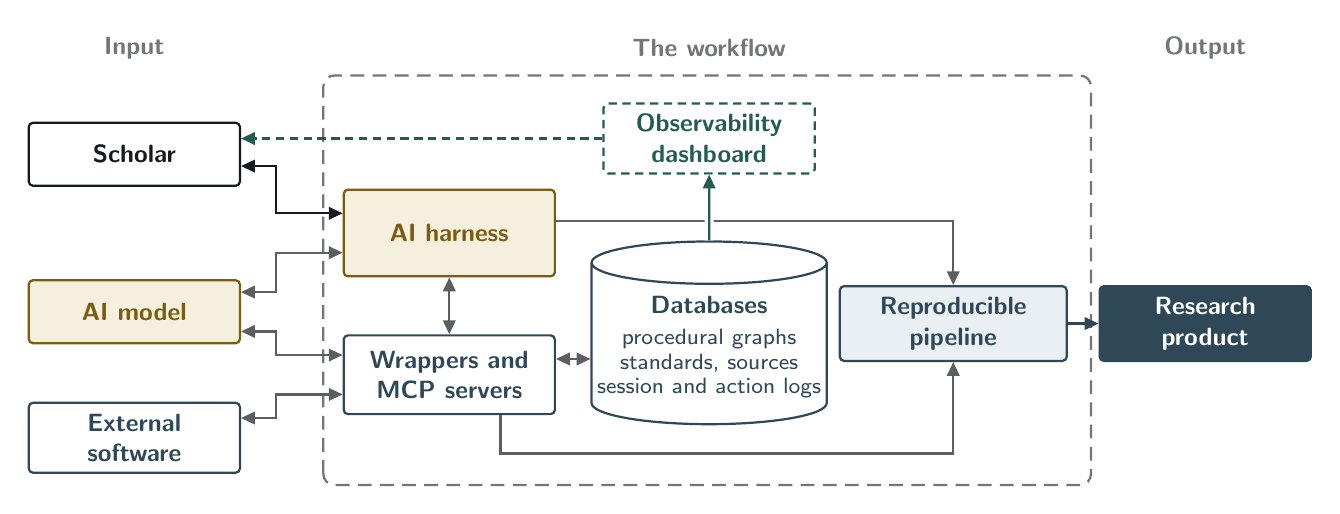
\begin{tikzpicture}
\tikzset{comp/.style={minimum width=2.6cm, minimum height=0.8cm, text width=2.4cm, font=\fontsize{9}{11}\selectfont\bfseries},
         edge/.style={<->, line width=0.8pt, cink!70},
         vlab/.style={font=\fontsize{8}{9.6}\selectfont, text=cink!80, inner sep=1.5pt},
         head/.style={font=\fontsize{9}{11}\selectfont\bfseries, text=cink!60}}
% column headings
\node[head] at (1.6,2.95) {Input};
\node[head] at (8.9,2.95) {The workflow};
\node[head] at (15.2,2.95) {Output};
% system boundary
\draw[cink!60, line width=0.8pt, dash pattern=on 5pt off 3pt, rounded corners=4pt] (4.0,-2.6) rectangle (13.75,2.6);
% input column
\node[person, comp] (sch) at (1.6,1.6) {Scholar};
\node[ai, comp] (model) at (1.6,-0.4) {AI model};
\node[pipe, comp, fill=white] (ext) at (1.6,-2.0) {External software};
% workflow
\node[ai, comp, minimum height=1.1cm] (h) at (5.6,0.6) {AI harness};
\node[pipe, comp, fill=white, minimum height=1.0cm] (wr) at (5.6,-1.2) {Wrappers and MCP servers};
\node[box, draw=cgreen, fill=white, text=cgreen, dash pattern=on 3pt off 2pt, comp] (dash) at (8.9,1.8) {Observability dashboard};
\node[cylinder, shape border rotate=90, aspect=0.18, draw=cslate, fill=white, line width=0.8pt, minimum width=2.7cm, minimum height=1.85cm, text=cslate, inner sep=2pt] (db) at (8.9,-0.85)
  {\begin{tabular}{@{}c@{}}{\fontsize{9}{11}\selectfont\bfseries Databases}\\[-1pt]{\fontsize{8}{9.4}\selectfont procedural graphs}\\[-3pt]{\fontsize{8}{9.4}\selectfont standards, sources}\\[-3pt]{\fontsize{8}{9.4}\selectfont session and action logs}\end{tabular}};
\node[pipe, comp, minimum width=2.8cm, text width=2.6cm] (pipe) at (12.0,-0.55) {Reproducible pipeline};
% output
\node[prod, comp] (rp) at (15.2,-0.55) {Research product};
% connections
\draw[<->, line width=0.8pt, cink] (sch.east |- 0,1.45) -- (3.4,1.45) |- (h.west |- 0,0.85);
\draw[edge] (model.east |- 0,-0.15) -- (3.4,-0.15) |- (h.west |- 0,0.35);
\draw[edge] (model.east |- 0,-0.65) -- (3.4,-0.65) |- (wr.west |- 0,-0.95);
\draw[edge] (ext.east |- 0,-1.75) -- (3.4,-1.75) |- (wr.west |- 0,-1.45);
\draw[edge] (h.south) -- (wr.north);
\draw[edge] (wr.east |- 0,-1.0) -- (db.west |- 0,-1.0);
\draw[->, line width=0.8pt, cink!70] (h.east |- 0,0.75) -- (12.0,0.75) -- (pipe.north);
\draw[->, line width=0.8pt, cink!70] (6.25,0 |- wr.south) -- (6.25,-2.2) -- (12.0,-2.2) -- (pipe.south);
\draw[white, line width=3.2pt] (db.north) -- (dash.south);
\draw[->, line width=0.8pt, cgreen] (db.north) -- (dash.south);
\draw[->, line width=0.8pt, cgreen, dash pattern=on 3pt off 2pt] (dash.west |- 0,1.8) -- (sch.east |- 0,1.8);
\draw[flow, cslate] (pipe.east) -- (rp.west);
\end{tikzpicture}
\end{document}
